\chapter{{Outlook: research publications underway}}\label{Outlook}
In this chapter, I address the ongoing research projects I hope to complete by the end of year $2023$, which include: The low temperature baryongenesis originating in nonequilibrium of bottom flavor; Population of Higgs in the early Universe; Extra neutrino from microscopic processes after freeze-out; and Self-consistent relaxation rate for electron-positron plasma in the early Universe.%; Effective screening potential in QGP/hadronic plasma to study heavy particle condensation.
.

\subsection{{Possibility of bottom-catalyzed low temperature baryongenesis}}
From the PDG, the observed baryon-to-photon density ratio $\eta$ today is given by  $5.8\times10^{-10} \leqslant\eta\leqslant6.5\times10^{-10}$ \cite{ParticleDataGroup:2018ovx} where the $\eta=(6.12\pm0.04)\times10^{-10}$~\cite{ParticleDataGroup:2022pth} is used in our calculation. This observed value is the evidence of baryon asymmetry and quantifies the matter-antimatter asymmetry in the Universe. In the past, the small value of the baryon asymmetry could be interpreted as simply due to the initial conditions in the Universe. However, in the current standard cosmological model, the inflation can erase any pre-existing asymmetry between baryons and anti-baryons. In this case, we need baryogenesis to generate of excess of baryon number compared to anti-baryon number in order to create the observed baryon number today.

The precise epoch responsible for the observed matter genesis $\eta$  in the early Universe has not been established yet. 
Several mechanisms have been proposed to explain baryogenesis with investigations typically focusing on the temperature range between GUT phase transition $T_\mathrm{G}\simeq10^{16}\,\mathrm{GeV}$ and the electroweak phase transition near $T_\mathrm{W}\simeq130\,\mathrm{GeV}$~\cite{Kuzmin:1985mm,Kuzmin:1987wn,Arnold:1987mh,Kolb:1996jt,Riotto:1999yt,Nielsen:2001fy,Giudice:2003jh,Davidson:2008bu,Morrissey:2012db}.

In following section we present arguments that the Sakharov conditions~\cite{Sakharov:1967dj} for matter asymmetry to form also appear during QGP hadronization era near to $T_\mathrm{H}\simeq150\,\mathrm{MeV}$, and show the possibility that bottom catalyzed the baryongenesis.

\paragraph{Overview of Sakhraov conditions}

In 1967, the Soviet physicist Sakharov first formulated the three conditions necessary to permit baryongenesis in the early Universe~\cite{Sakharov:1967dj} and in 1991 he refined the three conditions as follows~\cite{Sakharov:1988vdp}:
\begin{itemize}
  \item Absence of baryonic charge conservation 
  \item Violation of CP-invariance
  \item Non-stationary conditions in absence of local thermodynamic equilibrium
\end{itemize}

%The first condition, a violation of baryon $B$, lepton $L$ number conservation coincident around hadronization era, needs future theoretical and experimental consideration, constrained by the experimental limit on  proton life span $\mathcal{O}(10^{32}\mathrm{y}$). The relevant thermal environment can be explored in the laboratory since $T_\mathrm{H}=150$\,MeV is readily available in relativistic heavy ion (RHI) collision experiments~\cite{Rafelski:2019twp}. However, $T_\mathrm{H}$  may not suffice for catalysis of baryogenesis~\cite{Kuzmin:1985mm,Kuzmin:1987wn,Arnold:1987mh}. The second Sakharov condition requiring $CP$ assures us that we can recognize a universal difference between matter and antimatter, thus one abundance can be enhanced compared to the other.


\noindent Since the inflation erases any initial asymmetry between baryons and anti-baryons, the first condition, a violation of baryon number $B$, must exist to have the present baryon asymmetry. The second Sakharov condition requiring $CP$ violation assures us that we can recognize a universal difference between matter and antimatter, thus one abundance can be enhanced compared to the other.


The third condition, departure from thermal equilibrium, is one of the important prerequisites for matter genesis, this is because it creates the arrow in time for the Universe. In general, the thermal equilibrium implies both chemical (abundance) equilibrium and kinetic (equipartition of energy) equilibrium. The observed baryon and lepton numbers cannot be generated in a full thermal (chemical and kinetic) equilibrium, because even if the required processes are occurring, the net effect is cancelled out by the equal number of back-reactions. We believe that the presence of chemical non-equilibrium is more relevant -- kinetic equilibrium is usually established much more quickly and has less impact on the actual particle abundances~\cite{Koch:1986ud,Birrell:2014gea}. 

Chemical non-equilibrium can be achieved by breaking the detailed balance between particle production reaction and annihilation/decay. 
When the Universe expands and temperature cools down, the production process slows down and is not able to keep up with decay reactions. Then the detailed balance is broken and creates the arrow in time for the Universe. In this case, the third condition of Sakharov can be interpreted as:
\begin{itemize}
  \item Non-stationary conditions in absence of detailed balance,
\end{itemize}
where the ideal thermodynamic equilibrium is generalized to the concept of detailed balance.  



%~~~~~~~~~~~~~~~~~~~~~~~~~~~~~~~~~~~~~~~~~~~~~~~~~

%\subsection{Possibility of bottom-catalyzed matter genesis}
%Given that the non-equilibrium of bottom flavor arises at relatively low QGP temperature allows the Sakharov conditions around QGP hadronization. In this section, our interest is to study what conditions in the primordial QGP-HG phase transition can yield the observed baryon asymmetry today and provide the values for experiment investigation. 

 \paragraph{Is there enough bottom flavor to matter?} Considering that FLRW-Universe evolves conserving entropy, and that baryon and lepton number following on the era of matter genesis is conserved, the current day baryon $B$ to entropy $S$, $B/S$-ratio must be achieved during matter genesis. The estimates of present day baryon-to-photon density ratio $\eta$ allows the determination of the present value of baryon per entropy ratio \cite{Rafelski:2019twp,Letessier:2002ony,Fromerth:2002wb,Fromerth:2012fe}:
\begin{align}
\left(\frac{B}{S}\right)_{t_0}\!\!\!\!=\eta\left(\frac{n_\gamma}{\sigma_\gamma+\sigma_\nu}\right)_{\!t_0}\!\!\!\!=(8.69\pm0.05)\!\!\times\!\!10^{-11},
\end{align}
where the subscript $t_0$ denotes the present day value, where $\eta=(6.12\pm0.04)\times10^{-10}$~\cite{ParticleDataGroup:2018ovx} is used in calculation. Here we consider that the Universe today is dominated by photons and free-streaming low mass neutrinos~\cite{Birrell:2012gg}, and $\sigma_\gamma$ and $\sigma_\nu$ are the entropy density for photons and neutrinos, respectively. 
 
In chemical equilibrium the ratio of bottom quark (pair) density $n_b^{th}$ to entropy density $\sigma=S/V$ just above quark-gluon hadronization temperature $T_\mathrm{H}=150\sim160\,\mathrm{MeV}$ is $n_b^{th}/\sigma=10^{-10}\sim10^{-13}$ (see Fig.~\ref{number_entropy_b002}). By studying the bottom density per entropy near to the hadronization temperature and comparing it to the baryon-per-entropy ratio $B/S$  we found there is sufficient abundance of bottom quarks for the proposed matter genesis mechanism to be relevant.


\paragraph{Non-stationary conditions in absence of detailed balance}
We have demonstrated that the bottom quark nonequliibrium occurs near to QGP phase transition around the temperature $T=0.3\sim0.15$ GeV in Fig.~\ref{fugacity_bc} and Fig.~\ref{NonFugacity}. We demonstrate that the competition between weak interaction decay and the strong interaction fusion processes is responsible for driving the bottom quark departure from the equilibrium in the early Universe. In all cases we see prolonged non-equilibrium which provides the arrow of time for baryongenesis.

%After formation, the heavy $b, \bar b$ quark can bind with any of the available lighter quarks. %Here, we assume that due to the enhanced binding effect of $\mathrm{B}_c^\pm$ all bottom $b$, $\bar b$ quarks are found in $\mathrm{B}_c^\pm$ eventually.
%Formation of a matter excess over antimatter at a relatively late Universe evolution period has the additional merit of depending on an experimentally accessible Universe evolution stage: Further insight can be derived from  experimental study of bottom flavor in RHI collisions, and  more generally, exploration of the  the properties of bottom flavored particles, including but not limited to the search for a specific baryon non-conservation mechanism.

\paragraph{Violation of $CP$-invariance}
In general, violation of $CP$ asymmetry can occur in the amplitudes of hadron decay. The weak interaction $CP$ violation arises from the components of Cabibbo-Kobayashi-Maskawa (CKM) matrix associated with quark-level transition amplitude and $CP$-violating phase.

Given that the non-equilibrium of bottom flavor arises at relatively low QGP temperature, the bottom quark decay occurs from preformed $\mathrm{B}_x$ meson states, $x=u,d,s,c$~\cite{Karsch:1987pv,Brambilla:2010vq,Aarts:2011sm,Brambilla:2017zei,Bazavov:2018wmo,Offler:2019eij}. These decays violate aside of the $CP$ symmetry, see for example~\cite{LHCb:2019jta,LHCb:2020vut}. The exploration of the here interesting $CP$ symmetry breaking in B$_c(b\bar c)$ decay is in progress~\cite{Tully:2019ltb,HFLAV:2019otj,ParticleDataGroup:2018ovx}. 
 Present measurements of $CP$-violation suggest that the CP asymmetry parameter is around $\delta_{CP}\approx10^{-3}$ ~\cite{ParticleDataGroup:2018ovx}.


\paragraph{Nonequilibrium bottom and baryon asymmetry}
 The off equilibrium phenomenon of bottom quark around the temperature range $T=0.3\sim0.15$ GeV can provide the non-chemical equilibrium condition for baryogenesis to occur in the primordial-QGP hadronization era. Furthermore, let us consider the scenario where all bottom quarks are confined within $B_c^\pm$ meson. In this case, the decay of charged mesons in the primordial-QGP can be a source of $CP$ violation. However, it remains uncertain whether the decay of $B_c^\pm$ mesons contributes to baryon violation. Our postulation is as follows: the baryon asymmetry is produced by the bottom quark disappearance via the irreversible decay of $B^\pm_c$ meson during the off-equilibrium process. Once a baryon symmetry exists in universe, it will also produce the asymmetry between leptons and anti-leptons which is similar to the baryon asymmetry by the $L=B$.

The heavy $B_c^\pm$ meson decay into multi-particles in plasma is associated with the irreversible process. This is because after decay the daughter particles can interact with plasma and distribute their energy to other particles and reach equilibrium with the plasma quickly. In this case the  energy required for the inverse reaction to produce $B_c^\pm$ meson is difficult to overcome and therefore we have an irreversible process for multi-particle decay in plasma.


The rapid $B_c^\pm$ decay and bottom reformation speed at picosecond scale assures that there are millions of individual microscopic processes involving bottom quark production and decay before and during the hadronization epoch of QGP. In this case, we have an Urca process for the bottom quark, i.e. a cycling reaction that produces the bottom quark which subsequently  disappears via the $B_c^\pm$ meson decay. The Urca process is a fundamental physical process  and has been studying the realms of in astrophysics and nuclear physics. In our case, for bottom quark as a example: at low temperature, the number of bottom quark cycling can be estimated as
\begin{align}
\left.\mathrm{C_{cycle}}\right|_{T=0.2\mathrm{GeV}}=\frac{\tau_H}{\tau_{B_c}}\approx2\times10^7,
\end{align}
where the lifespan of $B_c^\pm$ is  $\tau_{\mathrm{B}_c}\approx0.51\times10^{-12}\,\mathrm{sec}$ and at temperature $T=0.2$ GeV the Hubble time is $\tau_H=1/H=1.272\times10^{-5}$ sec. The Urca process plays a significant role by potentially amplifying any small and currently unobserved violation of baryon number associated with the bottom quark. The small baryon asymmetry is enhanced by the Urca-like process with cycling ${\tau^\ast_H}/{\tau_\ast}$ in the early Universe.
This amplification would be crucial for achieving the required strength for today's observation. 


Full understanding of the possibility for baryogenesis to occur in primordial-QGP hadronization still requires a detailed study of the relation between baryon asymmetry and irreversible process; we are working on it now. Here, our interest is to show that our results provide a strong  motivation to explore the physics of baryon nonconservation involving the bottomnium mesons or/and bottom quarks in thermal environment.

%%%%%%%%%%%%%%%%%%%%%%%%%%%%%%%%%%%%%%%%%%%%%%%
\subsection{{Population of Higgs in the early Universe}}
In our earlier study, the bottom $(b)$ quark abundance depends on the competition between the strong interaction fusion and weak interaction decay rates. This lead to the off equilibrium phenomenon of the bottom quark near the hadronization temperature. The same idea can be applied to other heavy particles in QGP. In following we focus on the Higgs abundance first and develop methods for future detailed study.

Considering the temperature range $10\,\mathrm{GeV}>T>1\,\mathrm{GeV}$ in the early Universe, the number density of the Higgs can be written as
\begin{align}
n_{H}=\frac{\Upsilon_H}{2\pi^2}T^3\left(\frac{m_H}{T}\right)^2 K_2(m_H/T),
\end{align}
where $\Upsilon_H$ is the Higgs fugacity parameter, and $m_H=125$ GeV is the mass of Higgs. In the temperature range we consider here, we have $m_H\gg T$ which allows us to consider the Boltzmann limit for the calculation of Higgs number density.
%%%%%%%%%%%%%%%%%%%%%%%%%%%%%%%%%%%%%%%%%%%%%%%%%%%%%%%%%%%%%%%%%%
\begin{figure}[ht]
\begin{center}
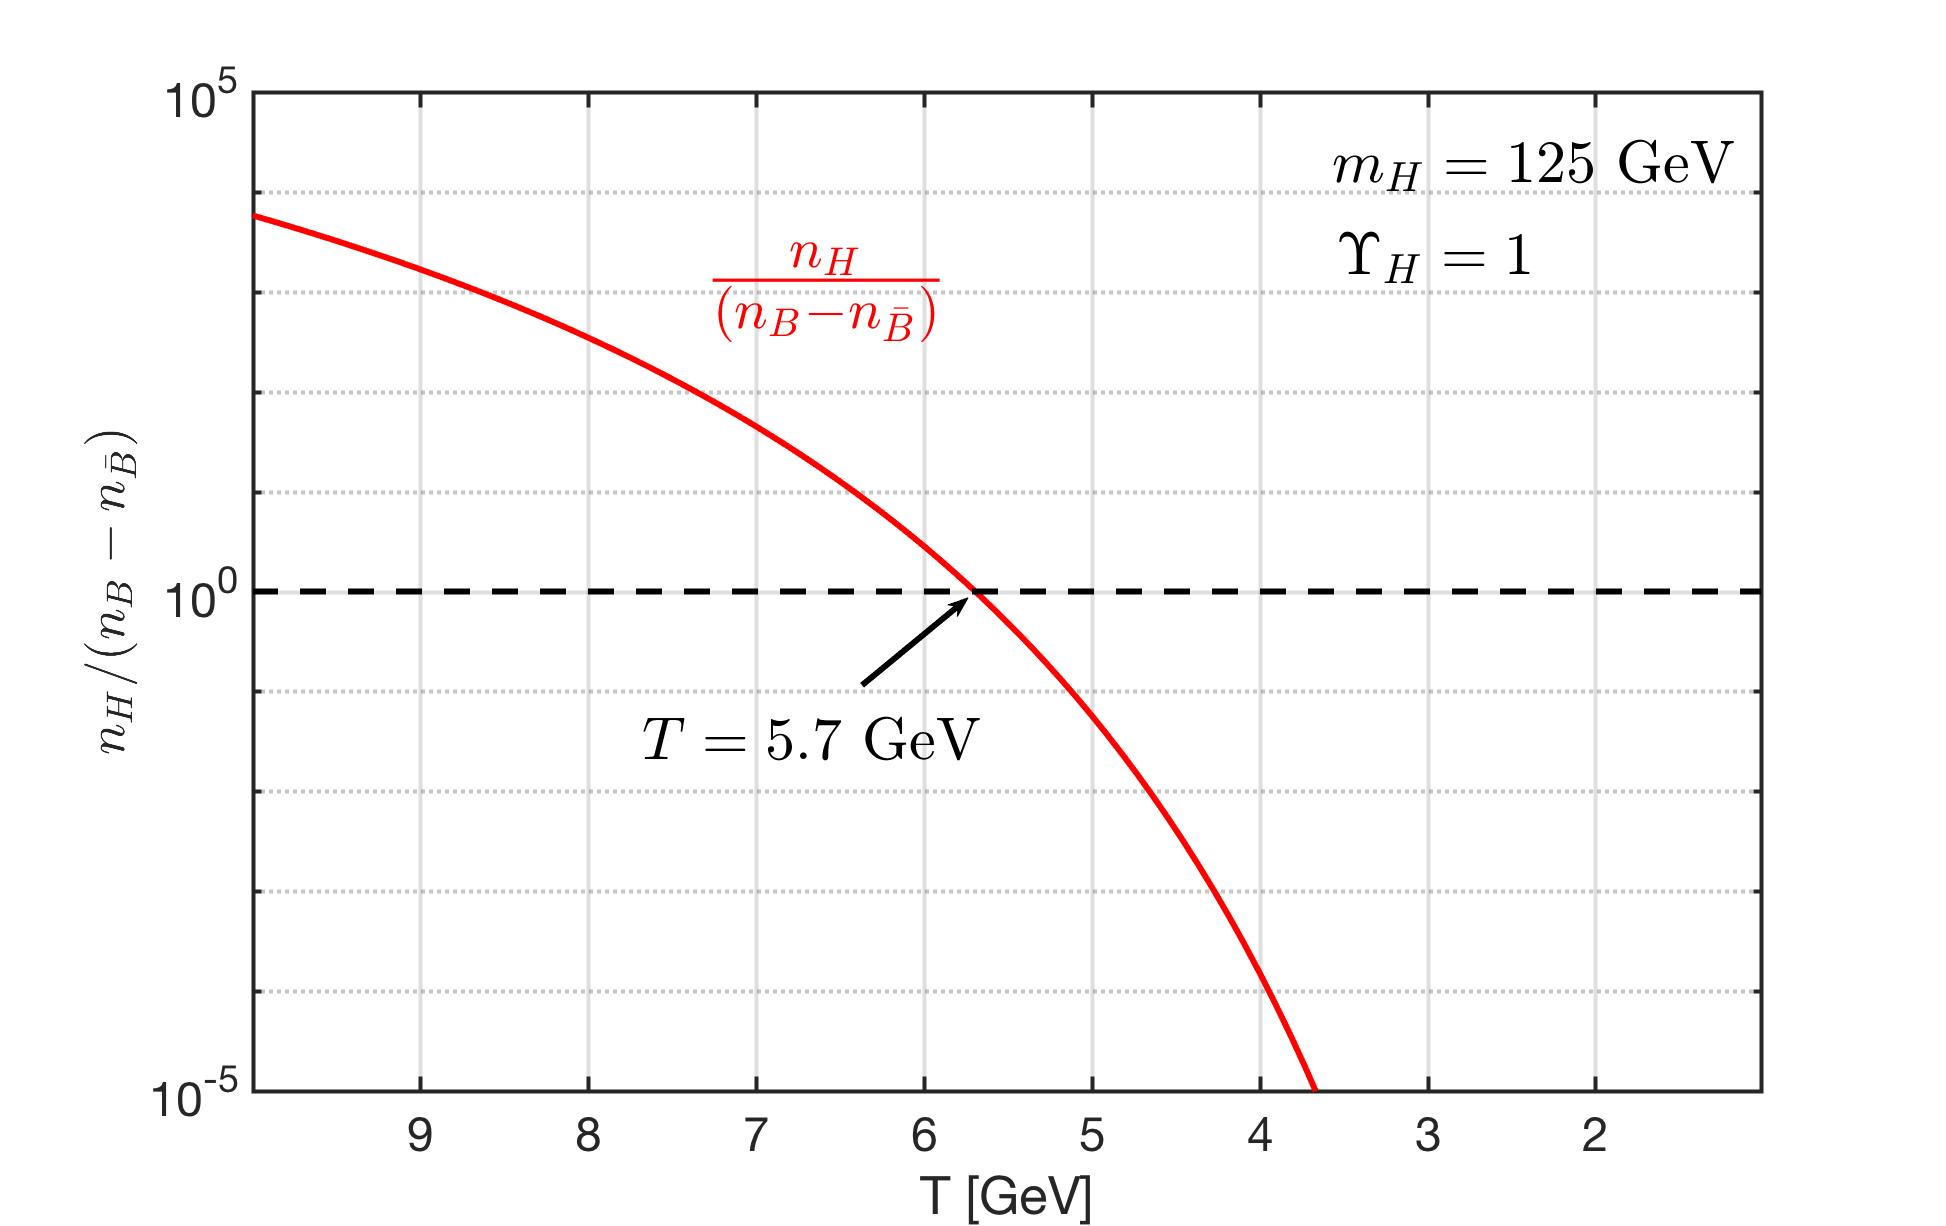
\includegraphics[width=\textwidth]{./plots/HiggsDensityRatio}
\caption{The density ratio between Higgs and baryon asymmetry as a function of temperature with condition $\Upsilon_H=1$. It shows that the $n_H=(n_B-n_{\bar{B}})$ at temperature $T=5.7$ GeV.}
\label{HiggsDensity_fig}
\end{center}
\end{figure}
%%%%%%%%%%%%%%%%%%%%%%%%%%%%%%%%%%%%%%%%%%%%%%%%%%%%%%%%%%%%%%%%%%%
Using constant baryon-per-entropy ratio, the density between Higgs and baryon asymmetry ($u,d$ quark-antiquark asymmetry) can be written as
\begin{align}
\frac{n_H}{(n_B-n_{\bar{B}})}=\frac{n_{H}}{s_{tot}}\,\left(\frac{s_{tot}}{n_B-n_{\bar{B}}}\right)=
\frac{n_{H}}{s_{tot}}\left(\frac{s_{\gamma,\nu}}{n_B-n_{\bar{B}}}\right)_{\!t_0},
\end{align}
where the present day value of baryon per entropy ratio is given by Eq.~(\ref{BaryonEntropyRatio}). The entropy density in QGP can be written as
\begin{align}
    &s_{tot}=\frac{2\pi^2}{45}g^s_\ast T_\gamma^3,\qquad g^s_\ast=\sum_{i=\mathrm{g},\gamma}g_i\left({\frac{T_i}{T_\gamma}}\right)^3+\frac{7}{8}\sum_{i=l^\pm,\nu,u,d}g_i\left({\frac{T_i}{T_\gamma}}\right)^3,
\end{align}
where we consider the massless particles in QGP only as a first estimation. In Fig.~\ref{HiggsDensity_fig}, we plot the density ratio between Higgs and baryon asymmetry for the case $\Upsilon_H=1$. It shows that at temperature $T=5.7$ GeV, the ratio is equal to one, i.e., $n_H=(n_B-n_{\bar{B}})$ which means that the Higgs abundance could influence baryon evolution because the Higgs number density is comparable to the baryon number density. This result motivated us to examine the Higgs boson and to study its dynamic abundance in detail during the QGP epoch.

In the QGP epoch, the dominant production of the Higgs boson is the bottom fusion reaction: 
\begin{align}
b+\overline{b}\longrightarrow H,
\end{align}
which is the inverse decay process of $H\to b+\overline{b}$. On the other hand, Higgs abundance disappears via the $W,Z$ decay channel as follows:
\begin{align}
H\longrightarrow WW^\ast, ZZ^\ast\longrightarrow\mathrm{anything}.
\end{align}
where $W^\ast,Z^\ast$ represent the virtual bosons. Once Higgs decays into the $W$ and $Z$ bosons, the short lifespan of $W,Z$ mean they decay into multi-particles and reequilibrate with the plasma quickly. In this case
the energy required for the inverse decay reaction to produce the Higgs boson is difficult to overcome in the temperature we are interested in. Similar to the case of bottom quark we studied, the competition between the production and decay of Higgs require the dynamic study of the particle abundance in the early Universe. We aim to apply the knowledge from our study of bottom quark to the Higgs boson, and to examine all other possible sources for Higgs production in QGP and developing methods for future study before the end of year 2023.






\subsection{{After neutrino freeze-out: Extra neutrinos from microscope processes}}

After neutrinos chemical freeze-out, the number of neutrinos is independently conserved. However, the presence of electron-positron rich plasma until $T=20$ keV permits the reaction $\gamma\gamma\to e^-e^+\to\nu\bar{\nu}$ to occur even after neutrinos decouple from the cosmic plasma. This suggests the small amount of extra neutrinos can be produced until temperature $T=20$ keV and can modify the free streaming distribution and the effective number of neutrinos. In this section, we examine the possible source of extra neutrino from electron-positron plasma and develop methods for
future detailed study.

Considering that neutrinos decouple at $T_f=2$ MeV and become free streaming after freeze-out. The presence of electron-positron plasma environment from $2\,\mathrm{MeV}>T>0.02$ MeV can allow the following weak reaction to occur:
\begin{align}
\gamma+\gamma\longrightarrow e^-+e^+\longrightarrow \nu+\bar{\nu}.
\end{align}
Given the  thermal reaction rate per volume $R_{\gamma\gamma\to e\overline{e}}$ for reaction $\gamma\gamma\to e\overline{e}$ and $R_{e\overline{e}\to\nu\overline{\nu}}$ for reaction $e\overline{e}\to\nu\overline{\nu}$, then the thermal reaction rate per volume for $\gamma\gamma\to e^-e^+\to\nu\bar{\nu}$ can be written as
\begin{align}
R_{\gamma\to e\to\nu}=R_{\gamma\gamma\to e\overline{e}}\left(\frac{R_{e\overline{e}\to\nu\overline{\nu}}}{R_{\gamma\gamma\to e\overline{e}}+R_{e\overline{e}\to\nu\overline{\nu}}}\right)\approx R_{e\overline{e}\to\nu\overline{\nu}}
\end{align}
In Fig.~\ref{ExtraNeutrinoRate} we plot the thermal reaction rate per volume for relevant reactions as a function of temperature $2\,\mathrm{MeV}>T>0.05\,\mathrm{MeV}$. It shows that the dominant reaction for the process $\gamma\gamma\to e^-e^+\to\nu\bar{\nu}$ is the $e\overline{e}\to\nu\overline{\nu}$ and can be approximated $R_{\gamma\to e\to\nu}=R_{e\overline{e}\to\nu\overline{\nu}}$ in the temperature we are interested in.
%%%%%%%%%%%%%%%%%%%%%%%%%%%%%%%%%%%%%%%%%%%%%%%%%%%%%%%%%%%%%%%%%%
\begin{figure}[ht]
\begin{center}
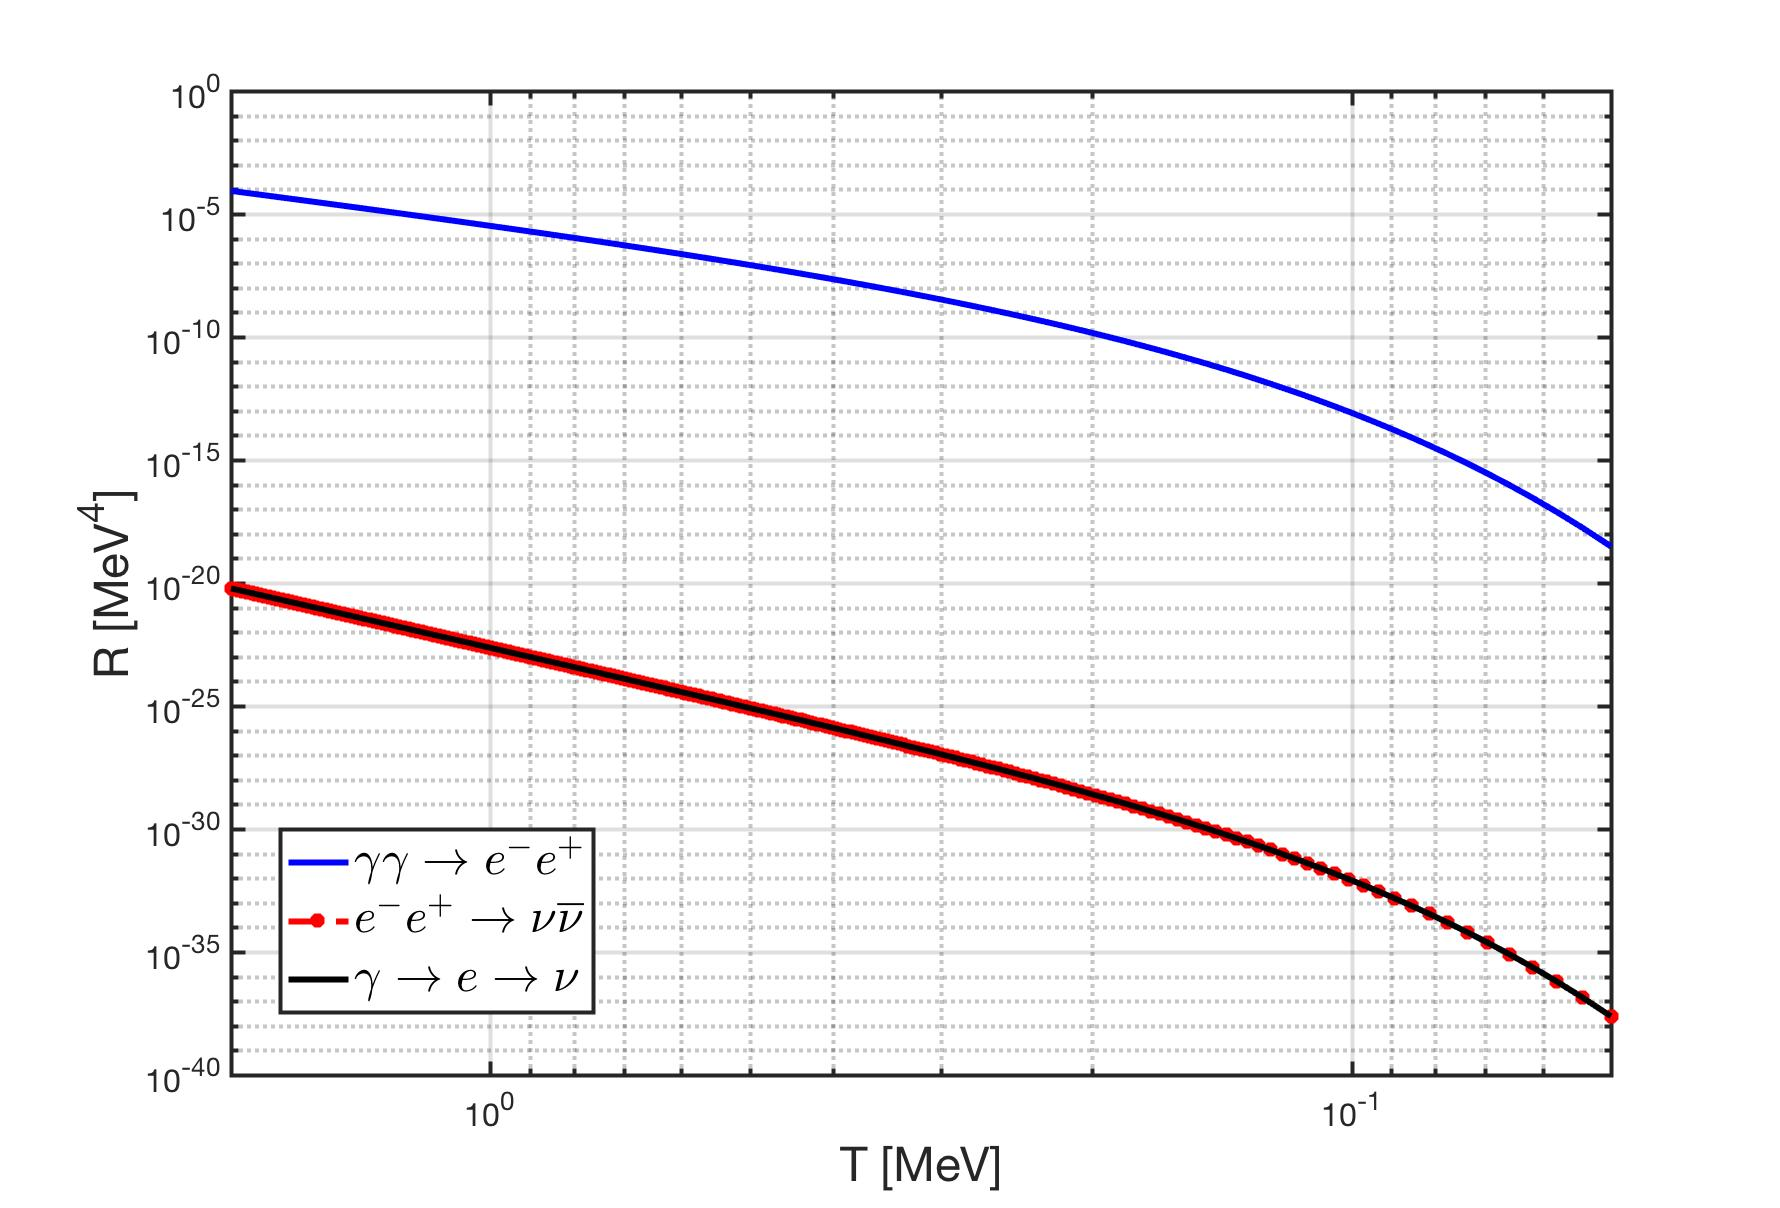
\includegraphics[width=\textwidth]{./plots/Extra_neutrino_rate_volume}
\caption{The thermal reaction rate per volume as a function of temperature $2\,\mathrm{MeV}>T>0.05\,\mathrm{MeV}$. The dominant reaction for the process $\gamma\gamma\to e^-e^+\to\nu\bar{\nu}$ is the $e\overline{e}\to\nu\overline{\nu}$ and we have $R_{\gamma\to e\to\nu}=R_{e\overline{e}\to\nu\overline{\nu}}$.}
\label{ExtraNeutrinoRate}
\end{center}
\end{figure}
%%%%%%%%%%%%%%%%%%%%%%%%%%%%%%%%%%%%%%%%%%%%%%%%%%%%%%%%%%%%%%%%%%%

Given the thermal reaction rate, the dynamic equation describing the relic neutrino abundance after freeze-out can be expressed as:
\begin{align}\label{ExtraNeutrio_eq}
\frac{dn_\nu}{dt}+3Hn_\nu=R_{e\overline{e}\to\nu\overline{\nu}}(T_{\gamma,e^\pm})-R_{\nu\overline{\nu}\to e\overline{e}}(T_\nu),
\end{align}
where $n_\nu$ is the number density of neutrinos and $H$ is the Hubble parameter. The parameter $T_{\gamma,e^\pm}$ is the equilibrium temperature between photons and $e^\pm$ and $T_\nu$ is the temperature for free-streaming neutrinos: 
\begin{align}
T_\nu=\frac{a(t_f)}{a(t)}T_f,
\end{align}
where $T_f$ is the neutrino freezeout temperature. After neutrinos decoupled from the cosmic plasma, we have $T_\nu\neq T_{\gamma,e^\pm}$. This is because
the conservation of entropy,  after freezeout, the relic neutrino entropy is conserved independently and the entropy from $e^\pm$ annihilation flows solely into photons and reheats the photons' temperature. However, after neutrino freezeout, extra entropy from electron-positron plasma can still flow into the free-streaming neutrino sector via the reaction $\gamma\gamma\to e^-e^+\to\nu\bar{\nu}$. To describe this novel situation, kinetic theory for entropy production needs to be adapted, a topic we will address in the future. Here we neglect this extra entropy and consider the standard scenario for first approximation.


In Fig.~\ref{DimensionlessRatio} we plot the temperature ratio $T_\nu/T_{\gamma,e^\pm}$, the rate ratio $R_{\nu\overline{\nu}\rightarrow e\overline{e}}/R_{e\overline{e}\rightarrow\nu\overline{\nu}}$ and $(R_{e\overline{e}\rightarrow\nu\overline{\nu}}-R_{\nu\overline{\nu}\rightarrow e\overline{e}})/R_{e\overline{e}\rightarrow\nu\overline{\nu}}$ as a function of temperature. It shows that after neutrino freezeout, the back reaction $\nu\overline{\nu}\rightarrow e\overline{e}$ becomes smaller compared to the reaction $e\overline{e}\rightarrow\nu\overline{\nu}$ as the temperature cools down. This is because as $T_\nu$ cools down, the density of relic neutrinos becomes so low and their energy becomes too small to interact. However, the hot and rich electron-positron plasma can still annihilate into neutrino pairs without any difficulties.
%%%%%%%%%%%%%%%%%%%%%%%%%%%%%%%%%%%%%%%%%%%%%%%%%%%%%%%%%%%%%%%%%
\begin{figure}[ht]
\begin{center}
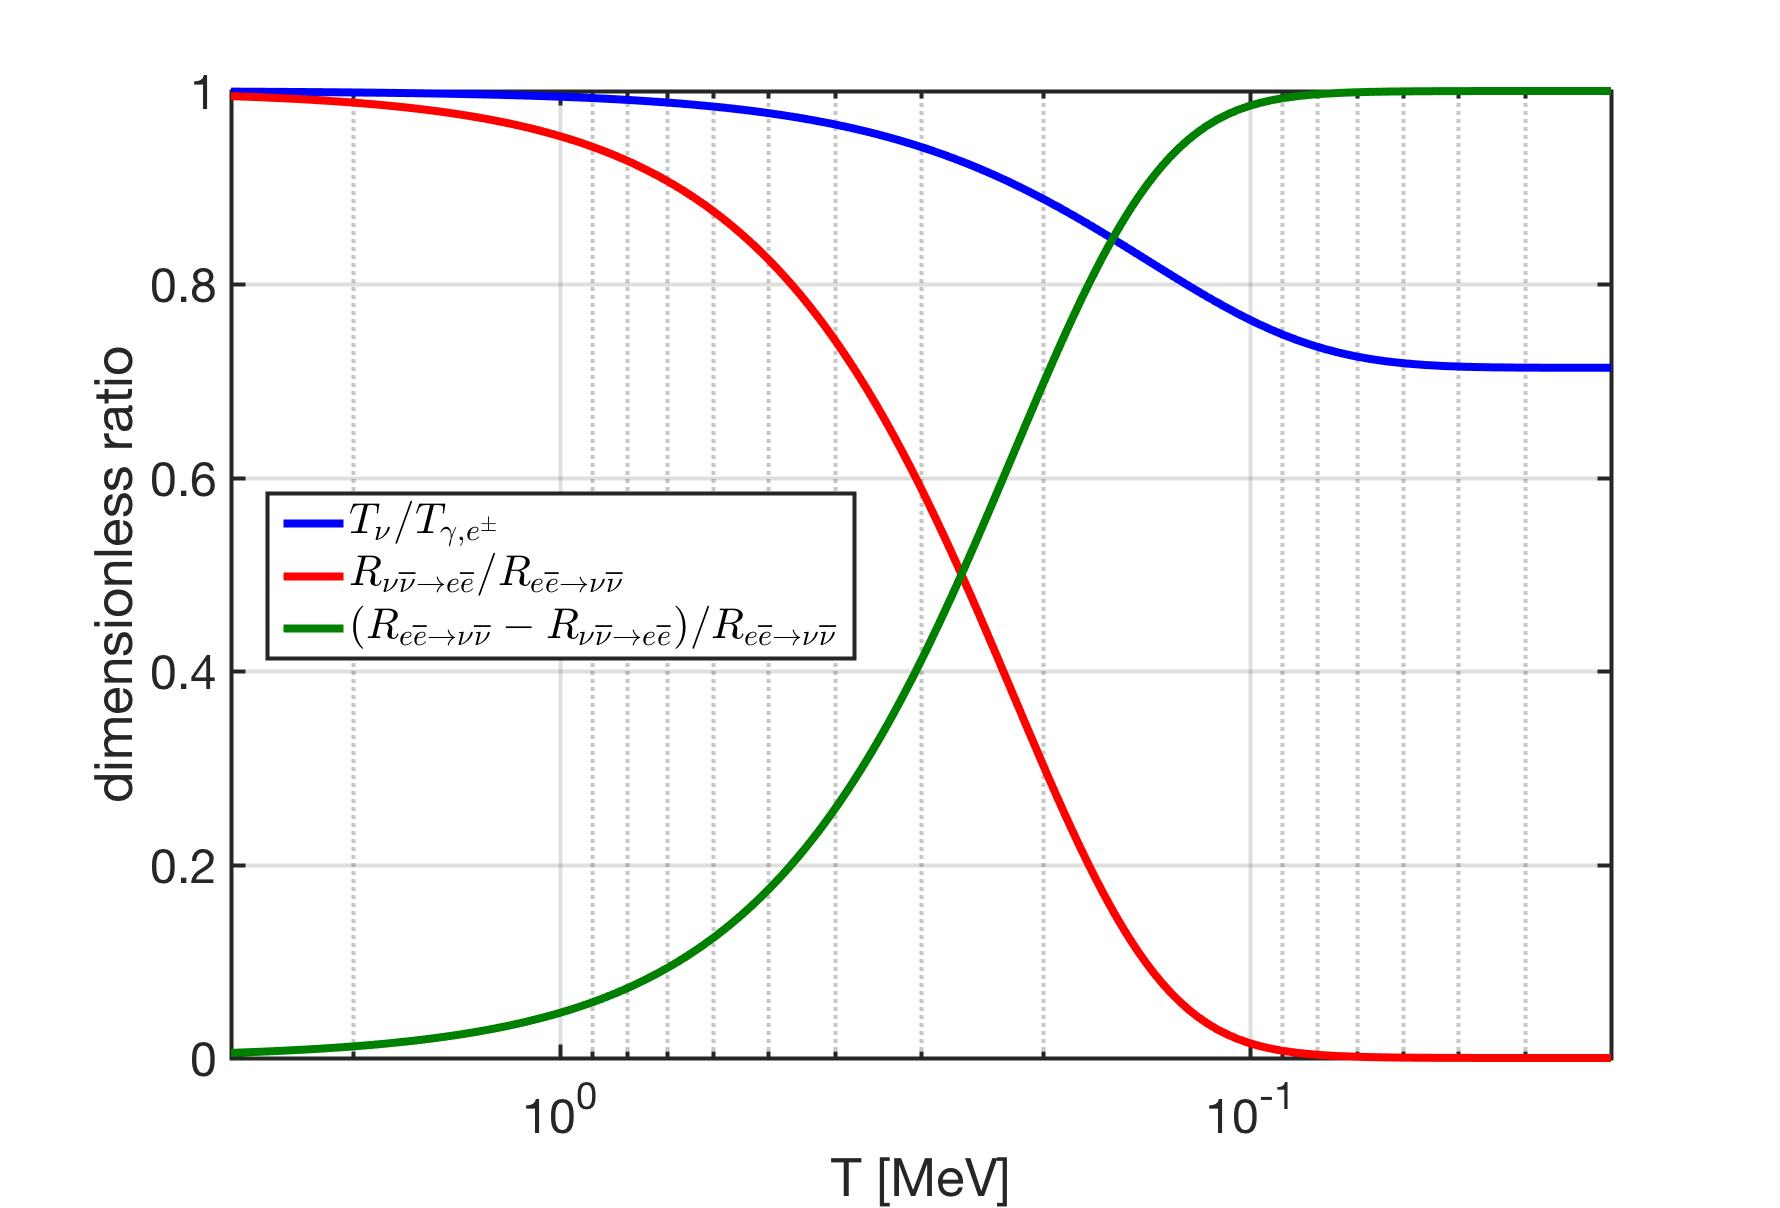
\includegraphics[width=\textwidth]{./plots/DimensionlessRatio_ExtraNeutrino}
\caption{The temperature ratio $T_\nu/T_{\gamma,e^\pm}$ (blue line), the rate ratio $R_{\nu\overline{\nu}\rightarrow e\overline{e}}/R_{e\overline{e}\rightarrow\nu\overline{\nu}}$ (red line) and $(R_{e\overline{e}\rightarrow\nu\overline{\nu}}-R_{\nu\overline{\nu}\rightarrow e\overline{e}})/R_{e\overline{e}\rightarrow\nu\overline{\nu}}$ (green line) as a function of temperature. It shows that the reaction $\nu\overline{\nu}\rightarrow e\overline{e}$ is small compare to the reaction $e\overline{e}\rightarrow\nu\overline{\nu}$ as temperature cooling down. }
\label{DimensionlessRatio}
\end{center}
\end{figure}
%%%%%%%%%%%%%%%%%%%%%%%%%%%%%
%%%%%%%%%%%%%%%%%%%%%%%%%%%%%%%%%%%%%%%%%%%%%%%%%%%

Solving the dynamic equation of neutrino abundance Eq.(\ref{ExtraNeutrio_eq}), the general solution can be written as
\begin{align}
n_\nu(T)=n_\mathrm{relic}(T)+n_\mathrm{extra}(T),\qquad T=T_{\gamma,e^\pm},
\end{align}
where $n_\mathrm{relic}$ represents the relic neutrino number density and $n_\mathrm{extra}$ is the extra number density from the $e^\pm$ annihilation. The relic neutrino density is given by
\begin{align}  &n_\mathrm{relic}=n_\nu^0\exp\left(-3\int_{t_i}^t{dt^\prime}H(t^\prime)\right)=n_\nu^0\exp\left(3\int_{T_i}^T\frac{dT^\prime}{T^\prime}(1+\mathcal{F})\right),\\
&n^0_\nu=g_\nu\frac{3\zeta(3)}{4\pi^2}T^3_i,\qquad F=\frac{T}{3g^\ast_s}\frac{dg^\ast_s}{dT},
\end{align}
where $T_i$ is the initial temperature and $g^\ast_s$ is the entropy degrees of freedom. The extra neutrino density can be written as
\begin{align}
n_\mathrm{extra}=-&\exp\left(3\int_{T_i}^T\frac{dT^\prime}{T^\prime}(1+\mathcal{F})\right)\notag\\
\times&\int_{T_i}^T\frac{dT^\prime}{T^\prime}\frac{R_{e\overline{e}}(T^\prime)-R_{\nu\overline{\nu}}(T^\prime_\nu)}{H(T^\prime)}\left(1+\mathcal{F}\right)\exp\left(-3\int_{T_i}^{T^{\prime}}\frac{dT^{\prime\prime}}{T^{\prime\prime}}(1+\mathcal{F})\right).
\end{align}
%%%%%%%%%%%%%%%%%%%%%%%%%%%%%%%%%%%%%%%%%%%%%%%%%%%%%%%%%%%%%%%%%%
\begin{figure}[ht]
\begin{center}
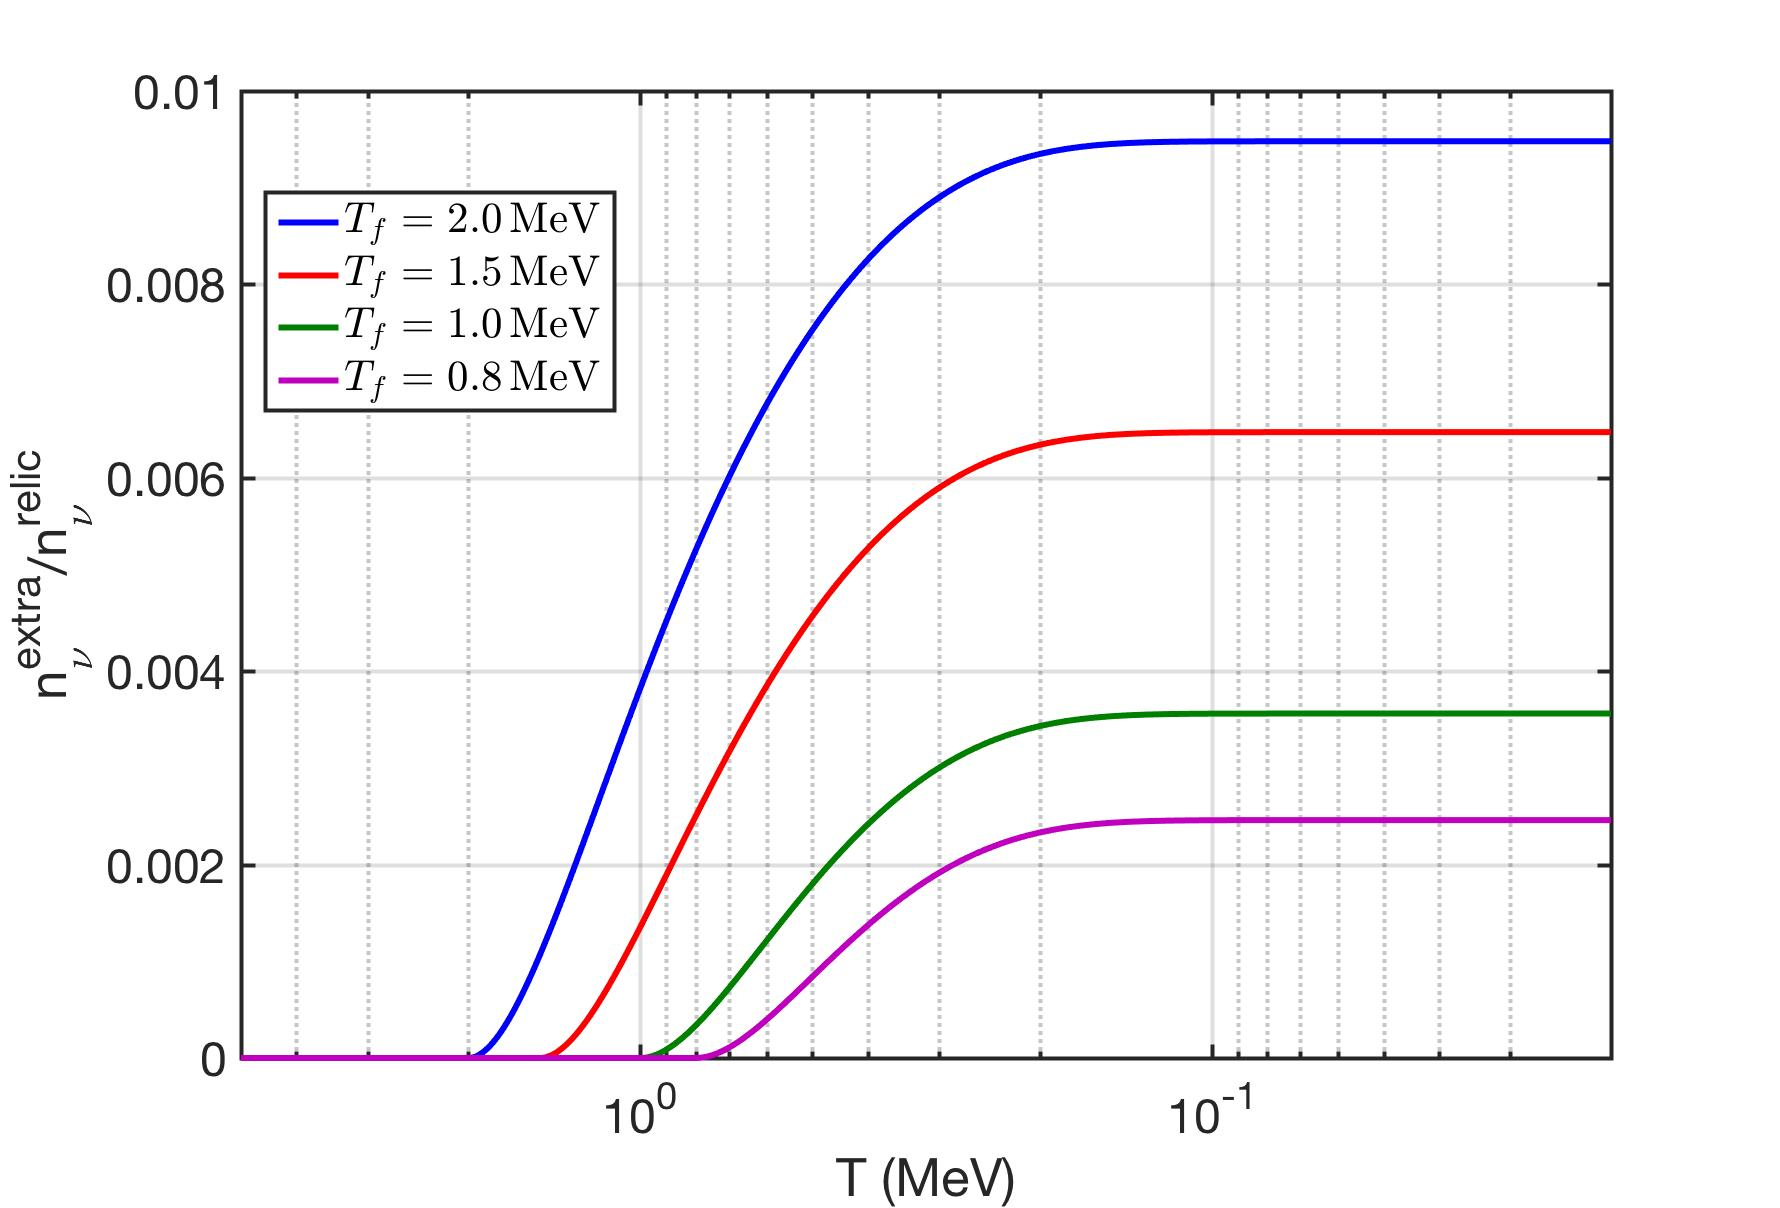
\includegraphics[width=\textwidth]{./plots/ExtraNeutrinoRatio}
\caption{the ratio between $n_{extra}/n_{relic}$ as a function of temperature with different neutrino freezeout temperature $T_f$. It shows that the higher freezeout temperature $T_f$ the higher number of extra neutrinos can be produced.}
\label{ExtraNeutrinoRatio}
\end{center}
\end{figure}
%%%%%%%%%%%%%%%%%%%%%%%%%%%%%%%%%%%%%%%%%%%%%%%%%%%%%%%%%%%%%%%%%%%

In Fig.~\ref{ExtraNeutrinoRatio} we plot the ratio between $n_\mathrm{extra}/n_\mathrm{relic}$ as a function of temperature with different neutrino freeze-out temperature $T_f$. It shows that the number of extra neutrinos depends strongly on the parameter $T_f$. This is because the freeze-out temperature determines the timing of the entropy transfer between $e^\pm$ and photon, which subsequently affects the evolution of temperature ratio between neutrinos and photons in the early Universe. The temperature ratio affects the rate ratio between $\nu\overline{\nu}\to e\overline{e}$ and $ e\overline{e}\to\nu\overline{\nu}$, because once the neutrino is too cold and the back reaction $\nu\overline{\nu}\to e\overline{e}$ can not maintain the balance, the $e^\pm$ annihilation starts to feed the extra neutrinos to the relic neutrino background. 

In addition to the annihilation of electron-positron pairs, there are other sources that can contribute to the presence of extra neutrinos in the early Universe. These additional sources include particle physics phenomena and plasma effects: neutrinos from charged leptons $\mu^\pm,\tau^\pm$ decay, neutrinos from the $\pi^\pm$ decay, and neutrino radiation from massive photon decay in electron-positron rich plasma. All of these potential sources of extra neutrinos can impact the distribution of freely streaming neutrinos and the effective number of neutrinos. Understanding these effects is crucial to comprehending how the neutrino component influences the expansion of the Universe, as well as the potential implications for large-scale structure formation and the spectrum of relic neutrinos.

\subsection{The $e^\pm$ plasma relaxation rate: Self-consistence approach}
In electron-positron plasma, the photon mass appears as $m_\gamma^2$ in the transition matrices for M{\o}ller and Bhabha reactions, which is one of important parameters in the calculation of the relaxation rate in $e^\pm$ plasma. When evaluating M{\o}ller and Bhabha scattering, we include the temperature-dependent mass of the photon obtained in plasma theory without damping. In general, the effective mass of the photon depends on the property of the plasma. Considering the linear response theory, the dispersion relation for the photon in nonrelativistic $e^\pm$ plasma is given by~\cite{Formanek:2021blc}
\begin{align}\label{dispersion_damping}
w^2=|k|^2+\frac{w}{w+i\kappa}w_{pl}^2,
\end{align}
where $w_{pl}$ is the plasma frequency and $\kappa$ is the average collision rate of $e^\pm$ plasma. The effective plasma frequency in damped plasma can be solved by considering the case $|k|^2=0$~\cite{Formanek:2021blc}
\begin{align}\label{plasmafrequency_damped}
w_{\pm}=-i\frac{\kappa}{2}\pm\sqrt{w^2_{pl}-\frac{\kappa^2}{4}}.
\end{align}
It shows that the plasma frequency in damped plasma $w_\pm$ is a function of $\kappa.$  In this case, the effective photon mass in damped plasma is also a function of the scattering rate. We have
\begin{align}\label{PhotonMass_self}
m_\gamma=w_\pm(w_{pl},\kappa)=m_\gamma(w_{pl},\kappa),
\end{align}
where the photon mass $m_\gamma=w_+$ for the underdamped plasma $w_{pl}>\kappa/2$, and $m_\gamma=w_-$ for overdamped plasma $w_{pl}<\kappa/2$. Eq.~(\ref{PhotonMass_self}) shows that computed damping strength $\kappa$ is the dominant scale for collisional plasma and it is also the main parameter determining the photon mass in plasma. 

Substituting the effective photon mass Eq.~(\ref{PhotonMass_self}) into the definition of the average relaxation rate Eq.~(\ref{Kappa}), we obtain the self-consistent equation for damping rate $\kappa$ as 
\begin{align}\label{RealaxtionSelf}
\kappa\,&\left[\frac{g_e}{2\pi^3}T^3\left(\frac{m_e}{T}\right)^2K_2(m_e/T)\right]\notag\\&=\frac{g_eg_e}{32\pi^4}T\!\!\int_{4m_e^2}^\infty\!\!\!\!ds\frac{s(s-4m^2_e)}{\sqrt{s}}K_1(\sqrt{s}/T)
\bigg[\sigma_{e^\pm e^\pm}(s,w_{pl},\kappa)+\sigma_{e^\pm e^\mp}(s,w_{pl},\kappa)\bigg],
\end{align}
where the cross sections depend on the parameter $w_{pl}$ and $\kappa$, and the variable $\kappa$ appears on both sides of the equation so we need solve the equation numerically to determine the $\kappa$ value that satisfies this condition.

Depending on the nature of the plasma (overdamped or underdamped plasma), we can establish the photon mass in collision plasma based on two distinct conditions as follows:
\begin{itemize}
\item Case 1. The plasma frequency is larger than the collision rate $w_{pl}>\kappa/2$, we have
\begin{align}
m_\gamma=w_+=-i\frac{\kappa}{2}+\sqrt{w^2_{pl}-\frac{\kappa^2}{4}}.
\end{align}
\item Case 2. The plasma frequency is smaller than the collision rate $w_{pl}<\kappa/2$, we have
\begin{align}\label{PhotonMassPlasma}
m_\gamma=w_-=-i\left(\frac{\kappa}{2}+\sqrt{\frac{\kappa^2}{4}-w^2_{pl}}\right).
\end{align}
\end{itemize}
In Fig.~\ref{RelaxationRate002_fig} it shows that during the BBN temperature range $50\leqslant T\leqslant 86$ keV, the plasma frequency is smaller than the collision rate $w_{pl}<\kappa/2$.  In this case, the effective photon mass in collision plasma during BBN epoch is given by Eq.(\ref{PhotonMassPlasma}).



%~~~~Figure~~~~~~~~~~~~~~~~~~~~~~~~~~~
\begin{figure}[h]
\begin{center}
%\includegraphics[width=0.95\linewidth]{KappaRateToT_May082023}
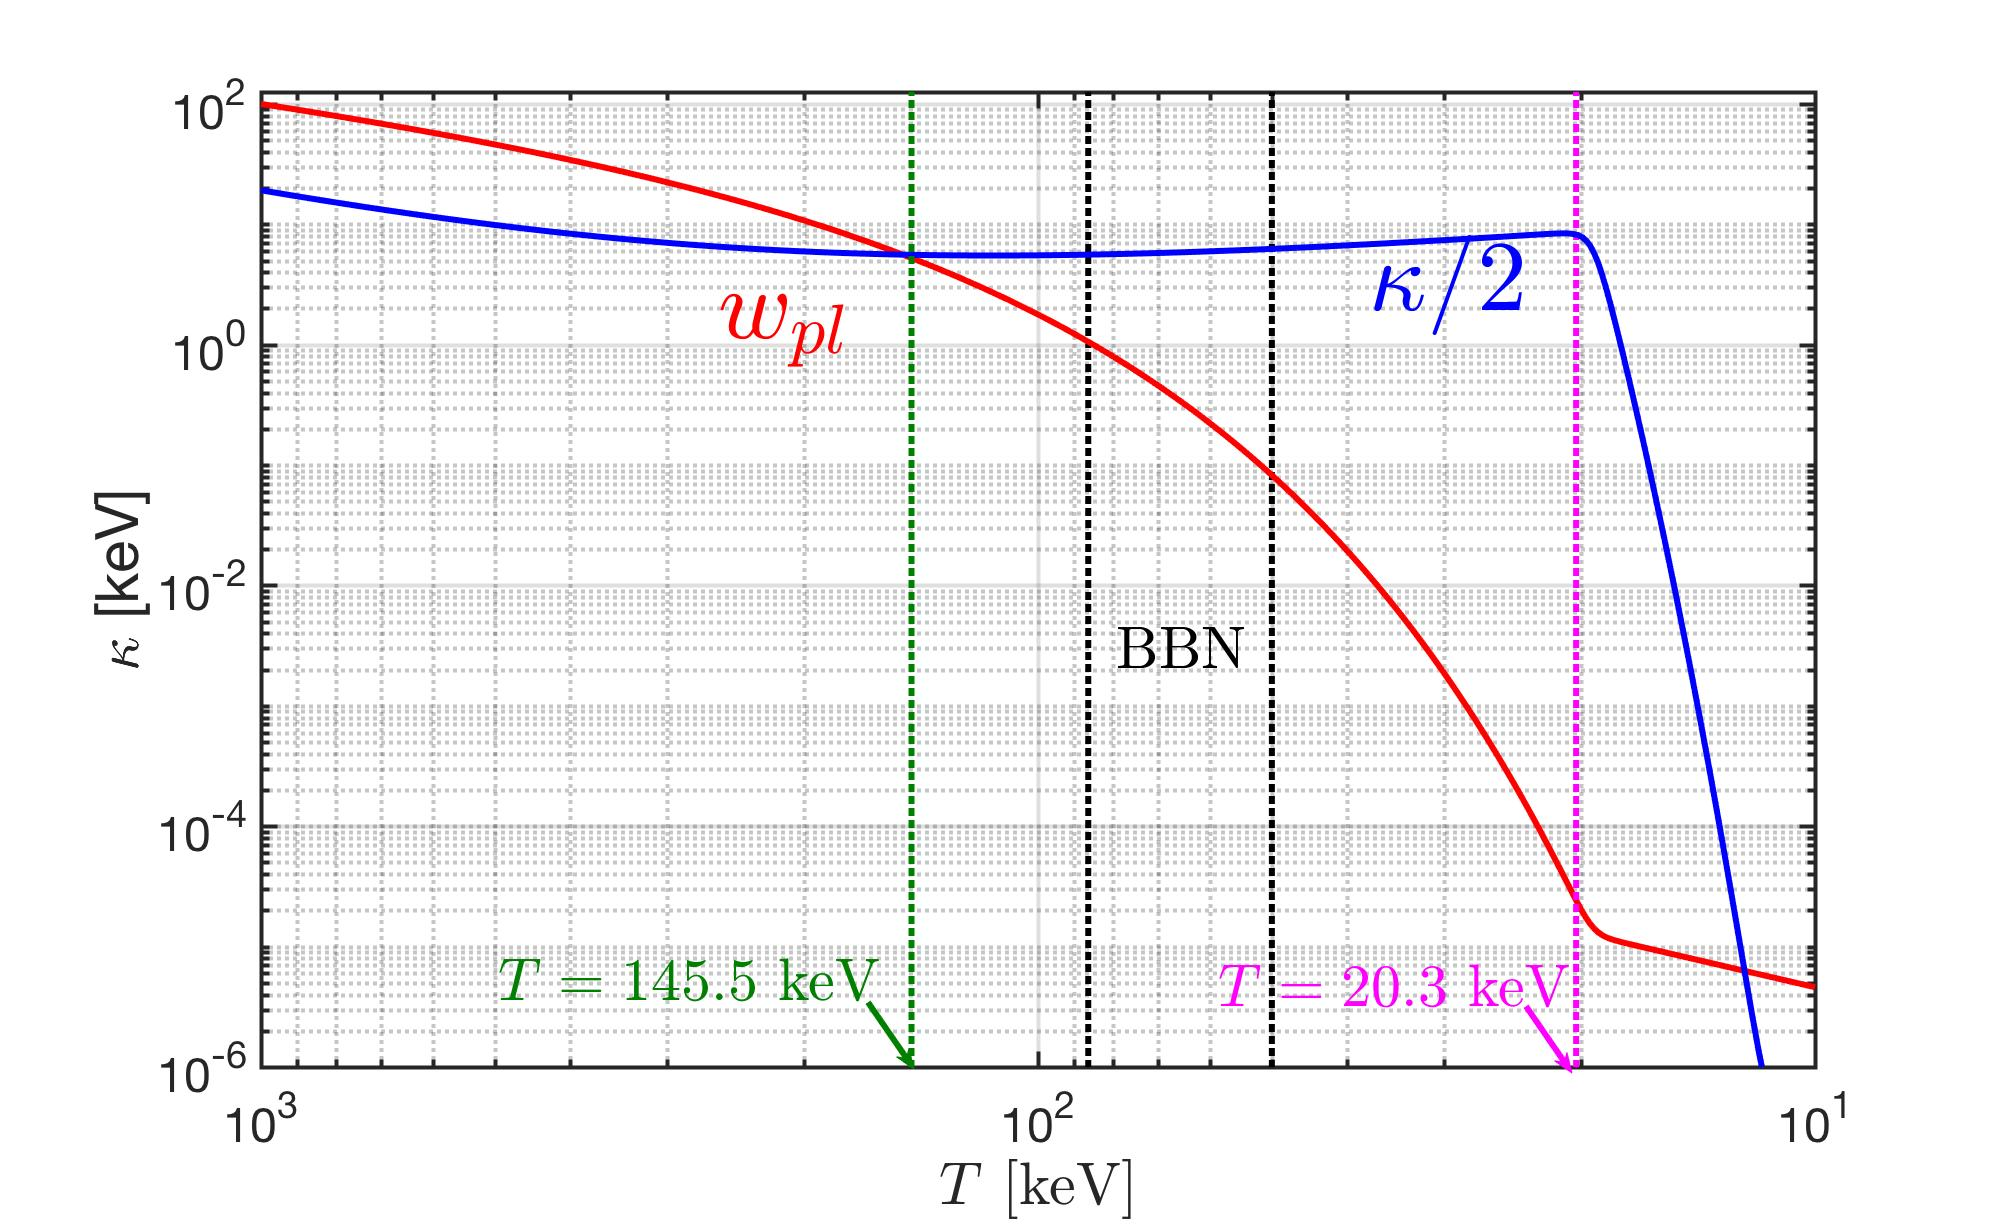
\includegraphics[width=\linewidth]{./plots/KappaElectronPhotonMass_Talk}
\caption{The relaxation rate $\kappa/2$ (blue line) as a function of temperature in nonrelativistic electron-positron plasma. For comparison, we show the plasma frequency $\omega_{pl}$ in the red line. It shows that for $T>145.5$ MeV, the plasma frequency is larger than the collision rate $w_{pl}>\kappa/2$; for temperature $T<145.5$ MeV, we have $\kappa/2>w_{pl}$. For temperature $T<20.3$ keV, the composition of plasma is changed to electron and proton, which is beyond our current study because of unequal numbers of electrons and positrons.}
\label{RelaxationRate002_fig}
\end{center}
\end{figure}
%~~~~Figure~~~~~~~~~~~~~~~~~~~~~~~~~~~

To calculate the cross section for  M{\o}ller and Bhabha scattering we need to include the imaginary photon mass in the calculation of transition matrix elements. In general, the real part of photon mass in the calculation includes the effective photon-electron/positron scattering in plasma, and the imaginary part of photon mass contributes to the decay width of massive photon in plasma. To estimate the effect of photon mass on the damping rate $\kappa$, we first consider the effective mass corresponding to photon-electron/positron scattering in plasma, and leave the photon decay for future study.

For BBN temperature $50\leqslant T\leqslant 86$ keV,
we have $w_{pl}<\kappa$ and the effective photon mass can be approximated as
\begin{align}
m^2_\gamma=w_-w_-^\ast&=\left(\frac{\kappa}{2}+\sqrt{\frac{\kappa^2}{4}-w^2_{pl}}\right)^2
=\frac{\kappa^2}{2}\left[\left(1-\frac{2w^2_{pl}}{\kappa^2}\right)+\sqrt{1-\frac{4w^2_{pl}}{\kappa^2}}\right]\notag\\
&=\frac{\kappa^2}{2}\left[\left(1-\frac{2w^2_{pl}}{\kappa^2}\right)+\left(1-\frac{2w^2_{pl}}{\kappa^2}+\cdots\right)\right]\approx\kappa^2.
\label{PhotonMassPlasma002}
\end{align}
where we consider the limit $w^2_{pl}/\kappa^2\ll1$ and effective photon mass is equal to the average collision rate in plasma $m^2_\gamma\approx\kappa$.

Substituting the photon mass $m^2_\gamma=\kappa^2$ for overdamping plasma into the relaxation rate of electron-positron Eq.~(\ref{RealaxtionSelf}), and introducing the following dimensionless variables
\begin{align}
x=\sqrt{s}/T,\qquad a=m_\gamma/T=\kappa/T,\qquad b=m_e/T,
\end{align}
%~~~~~~~~~~~~~~~~~~~~~~~~~~~~~~~~~~~~~~~~~~~~~~~~~~~~~~~~~~~~~~~~~~~~~~~~~~~~~~~~
\begin{figure}[ht]
%\begin{center}
\centering
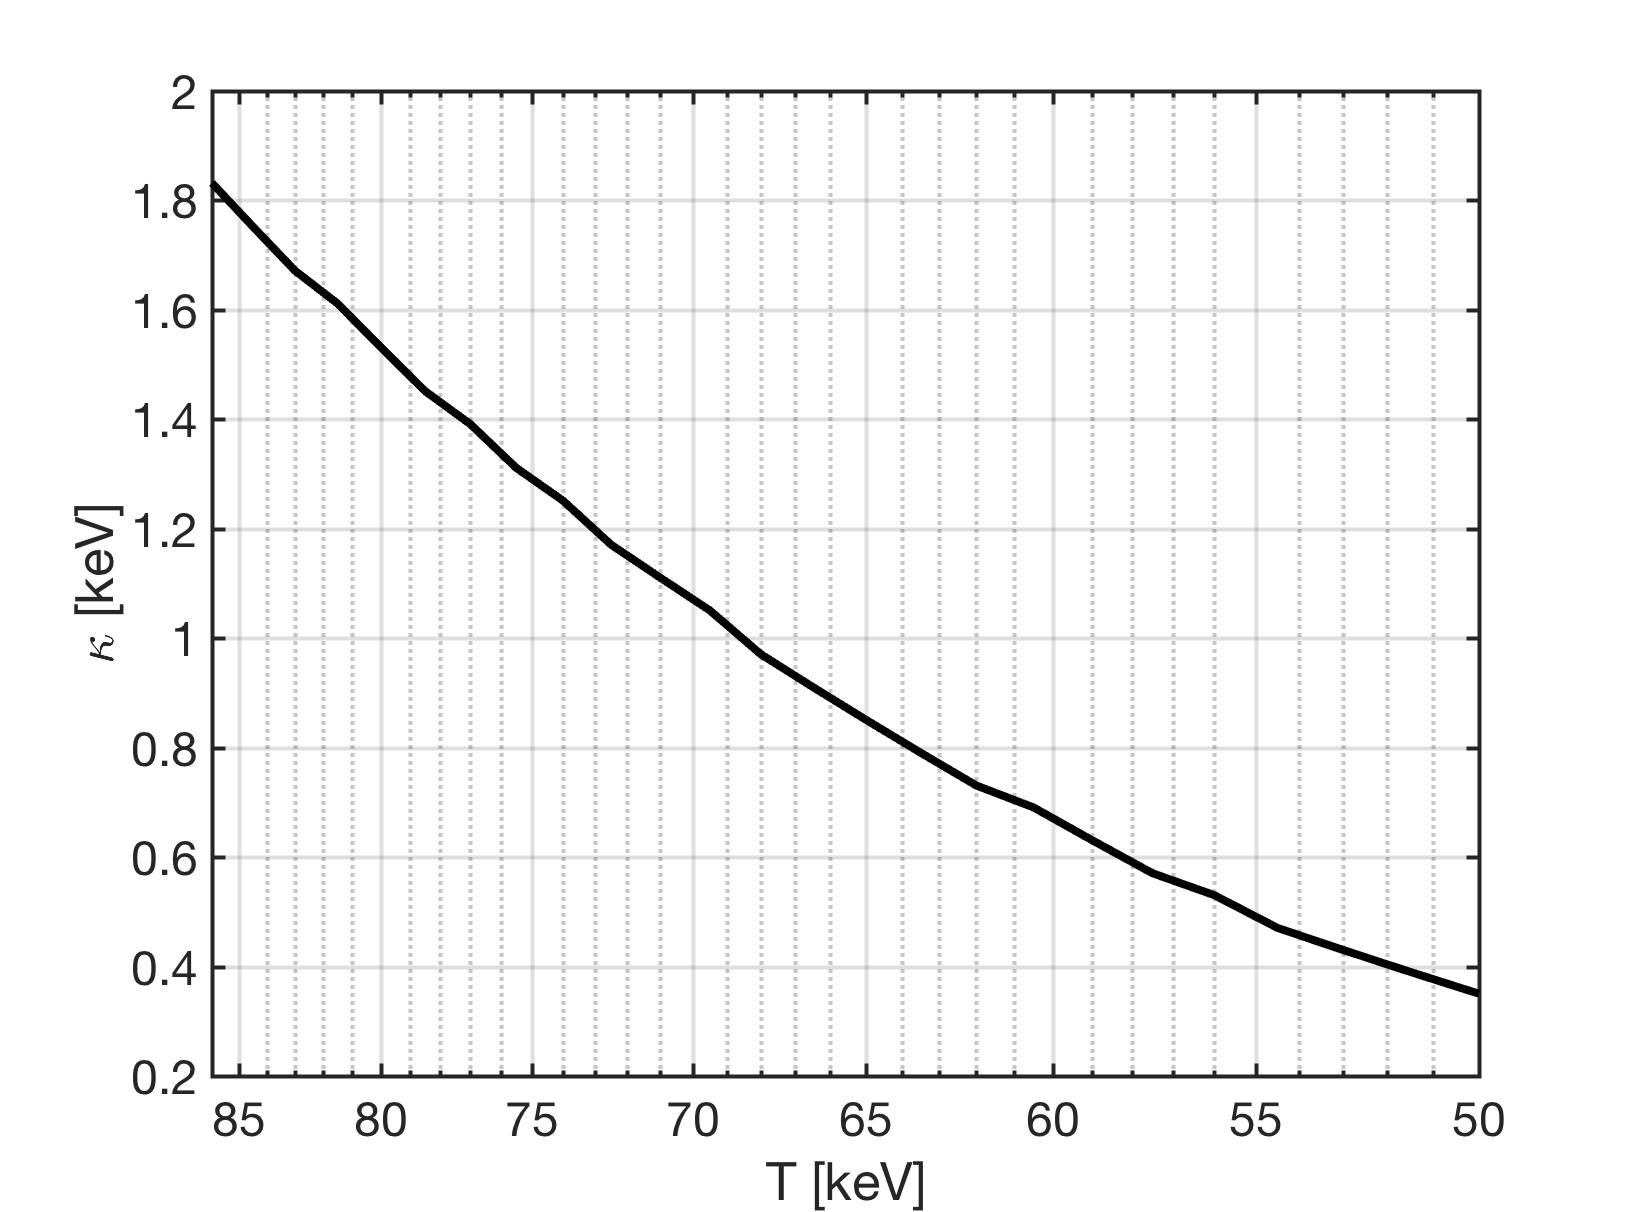
\includegraphics[width=\linewidth]{./plots/OverdampingKappa.jpg}
\caption{The relaxation rate $\kappa$ that satisfies Eq.(\ref{Numerical_eq}) as a function of temperature $50\leqslant T\leqslant 86$\,keV. It shows that for overdamping plasma, we have $m^2_\gamma=\kappa^2$, and $\kappa=1.832$\,keV when $T=86$\,keV and $\kappa=0.350$\,keV when $T=50$\,keV. The minor fluctuations are a result of the restricted numerical precision.}
\label{KappaSol.fig} 
\end{figure}
%~~~~~~~~~~~~~~~~~~~~~~~~~~~~~~~~~~~~~~~~~~~~~~~~~~~~~~~~~~~~~~~~~~~~~~~~~~~~~~~~
then the relaxation rate of electron-positron can be written as
\begin{align}\label{Numerical_eq}
&\left[\frac{g_e}{2\pi^2}T^4\left(\frac{m_e}{T}\right)^{\!2}\!K_2(m_e/T)\right]\,\left(\frac{\kappa}{T}\right)\notag\\
&\qquad\qquad\qquad=\frac{g^2_e\alpha^2}{8\pi^3}T^4\!\!\int_{2b}^\infty\!dxK_1(x)\left[\mathcal{F}_{e^\pm e^\pm}(x,\kappa/T)+\mathcal{F}_{e^\pm e^\mp}(x,\kappa/T)\right],
\end{align}
where the functions $\mathcal{F}_{e^\pm e^\pm}$ and $\mathcal{F}_{e^\pm e^\mp}$ are given by
\begin{align}
\mathcal{F}_{e^\pm e^\pm}(x,a=\kappa/T)&=\left\{2\left[3a^2+4b^2+\frac{4(b^4-a^4)}{x^2-4b^2+2a^2}\right]\ln\left(\frac{a^2}{x^2-4b^2+a^2}\right)\right.\notag\\
&\left.+\frac{(x^2-4b^2)(8b^4+2a^4+3a^2x^2+2x^4-4b^2(2x^2+a^2))}{a^2(x^2-4b^2+a^2)}\right\}
\end{align}
and 
\begin{align}
\mathcal{F}_{e^\pm e^\mp}(x,a=\kappa/T)&=\left\{\frac{2x^2(a^2+x^2)-4b^4}{x^2-a^2}\ln\left(\frac{a^2}{x^2-4b^2+a^2}\right)\right.\notag\\
&+\frac{(x^2-4b^2)(3x^2+4b^2+2a^2)}{(x^2-a^2)}+\frac{x^6-12b^4x^2-16b^6}{3(x^2-a^2)^2}\notag\\
&\left.+\frac{(x^2-4b^2)(8b^4+2a^4+3a^2x^2+2x^4-4b^2(2x^2+a^2))}{a^2(x^2-4b^2+a^2)}\!\right\}.
\end{align}

To determine the $\kappa$ that satisfies Eq.~(\ref{Numerical_eq}), we can solve it numerically. 
In Fig.~\ref{KappaSol.fig}, we plot the relaxation rate $\kappa$ that satisfies Eq.~(\ref{Numerical_eq}) as a function of temperature $50\,\mathrm{keV} \leqslant T\leqslant 86$ keV. It shows that during the BBN temperature range, we have overdamping electron/positron plasma $w_{pl}<\kappa$, and the effective photon mass $m^2_\gamma=\kappa^2$. The relaxation rate $\kappa=1.832\sim0.350$ keV during the BBN temperature range, which is smaller than the relaxation rate without damping photon mass (See Fig.~\ref{RelaxationRate_fig}, where the relaxation rate $\kappa=10\sim12$ keV during the BBN temperature).

Our first estimation implies that the relaxation rate is sensitive to the photon mass in damped plasma. To address the self-consistent evaluation of damping  rate in plasma requires the development of a well-defined, self-consistent approach, where both damping and photon properties in plasma are determined in a mutually consistent manner. We aim to include the full photon mass effect (both real and imaginary parts) in the study and improve our calculation for the next step to complete the project.

